%\title{Hierarchical Auxetic Elasticity}

%\author{Carlos Villarroel${}^{1}$}
%\affiliation{${}^1$Instituto de F\'isica, Pontificia Universidad Cat\'olica de Chile, Casilla 306, Santiago, Chile}

\documentclass[11pt,a4paper]{article}

% -----------------------------
% Idioma y codificación
% -----------------------------
\usepackage[spanish]{babel}
\usepackage[utf8]{inputenc}
\usepackage[T1]{fontenc}

% -----------------------------
% Matemática
% -----------------------------
\usepackage{amsmath,amssymb}

% -----------------------------
% Figuras
% -----------------------------
\usepackage{graphicx}
\usepackage{float}
\usepackage[font=footnotesize,labelfont=bf]{caption}

% -----------------------------
% Márgenes
% -----------------------------
\usepackage{geometry}
\geometry{
  left=2.5cm,
  right=2.5cm,
  top=2.5cm,
  bottom=2.5cm
}

% -----------------------------
% Espaciado
% -----------------------------
\usepackage{setspace}
\setstretch{1.15}

% -----------------------------
% Bibliografía
% -----------------------------
\usepackage[numbers]{natbib}

% -----------------------------
% Información del documento
% -----------------------------
\title{\textbf{Hierarchical Auxetic Elasticity}}
\author{
Carlos Villarroel$^{1}$ \\
\vspace{0.2cm}
\small $^{1}$Instituto de Física, Pontificia Universidad Católica de Chile, Santiago, Chile
}
\date{Septiembre 2026}

% -----------------------------
\begin{document}
% -----------------------------

\maketitle

% =================================================
\section{Modelo}
\label{sec:model}
% =================================================

Consideramos una estructura jerárquica construida a partir de cuadrados
rígidos conectados mediante bisagras. El nivel $i=0$ corresponde a un
cuadrado elemental, mientras que cada nivel siguiente se obtiene
ensamblando cuatro copias del nivel anterior, como se muestra en la
Fig.~\ref{fig:levels}. Una estructura de $N$ niveles contiene, por tanto,
$4^{N-i}$ unidades de nivel $i$.

La deformación se describe mediante las rotaciones de las unidades,
manteniendo rígidos los cuadrados elementales. En esta descripción
reducida, todas las copias de un mismo nivel comparten un único ángulo
$\theta_i$. Así, la configuración completa queda caracterizada por
los $N$ ángulos $\{\theta_i\}_{i=1}^{N}$.

\begin{figure}[H]
  \centering
  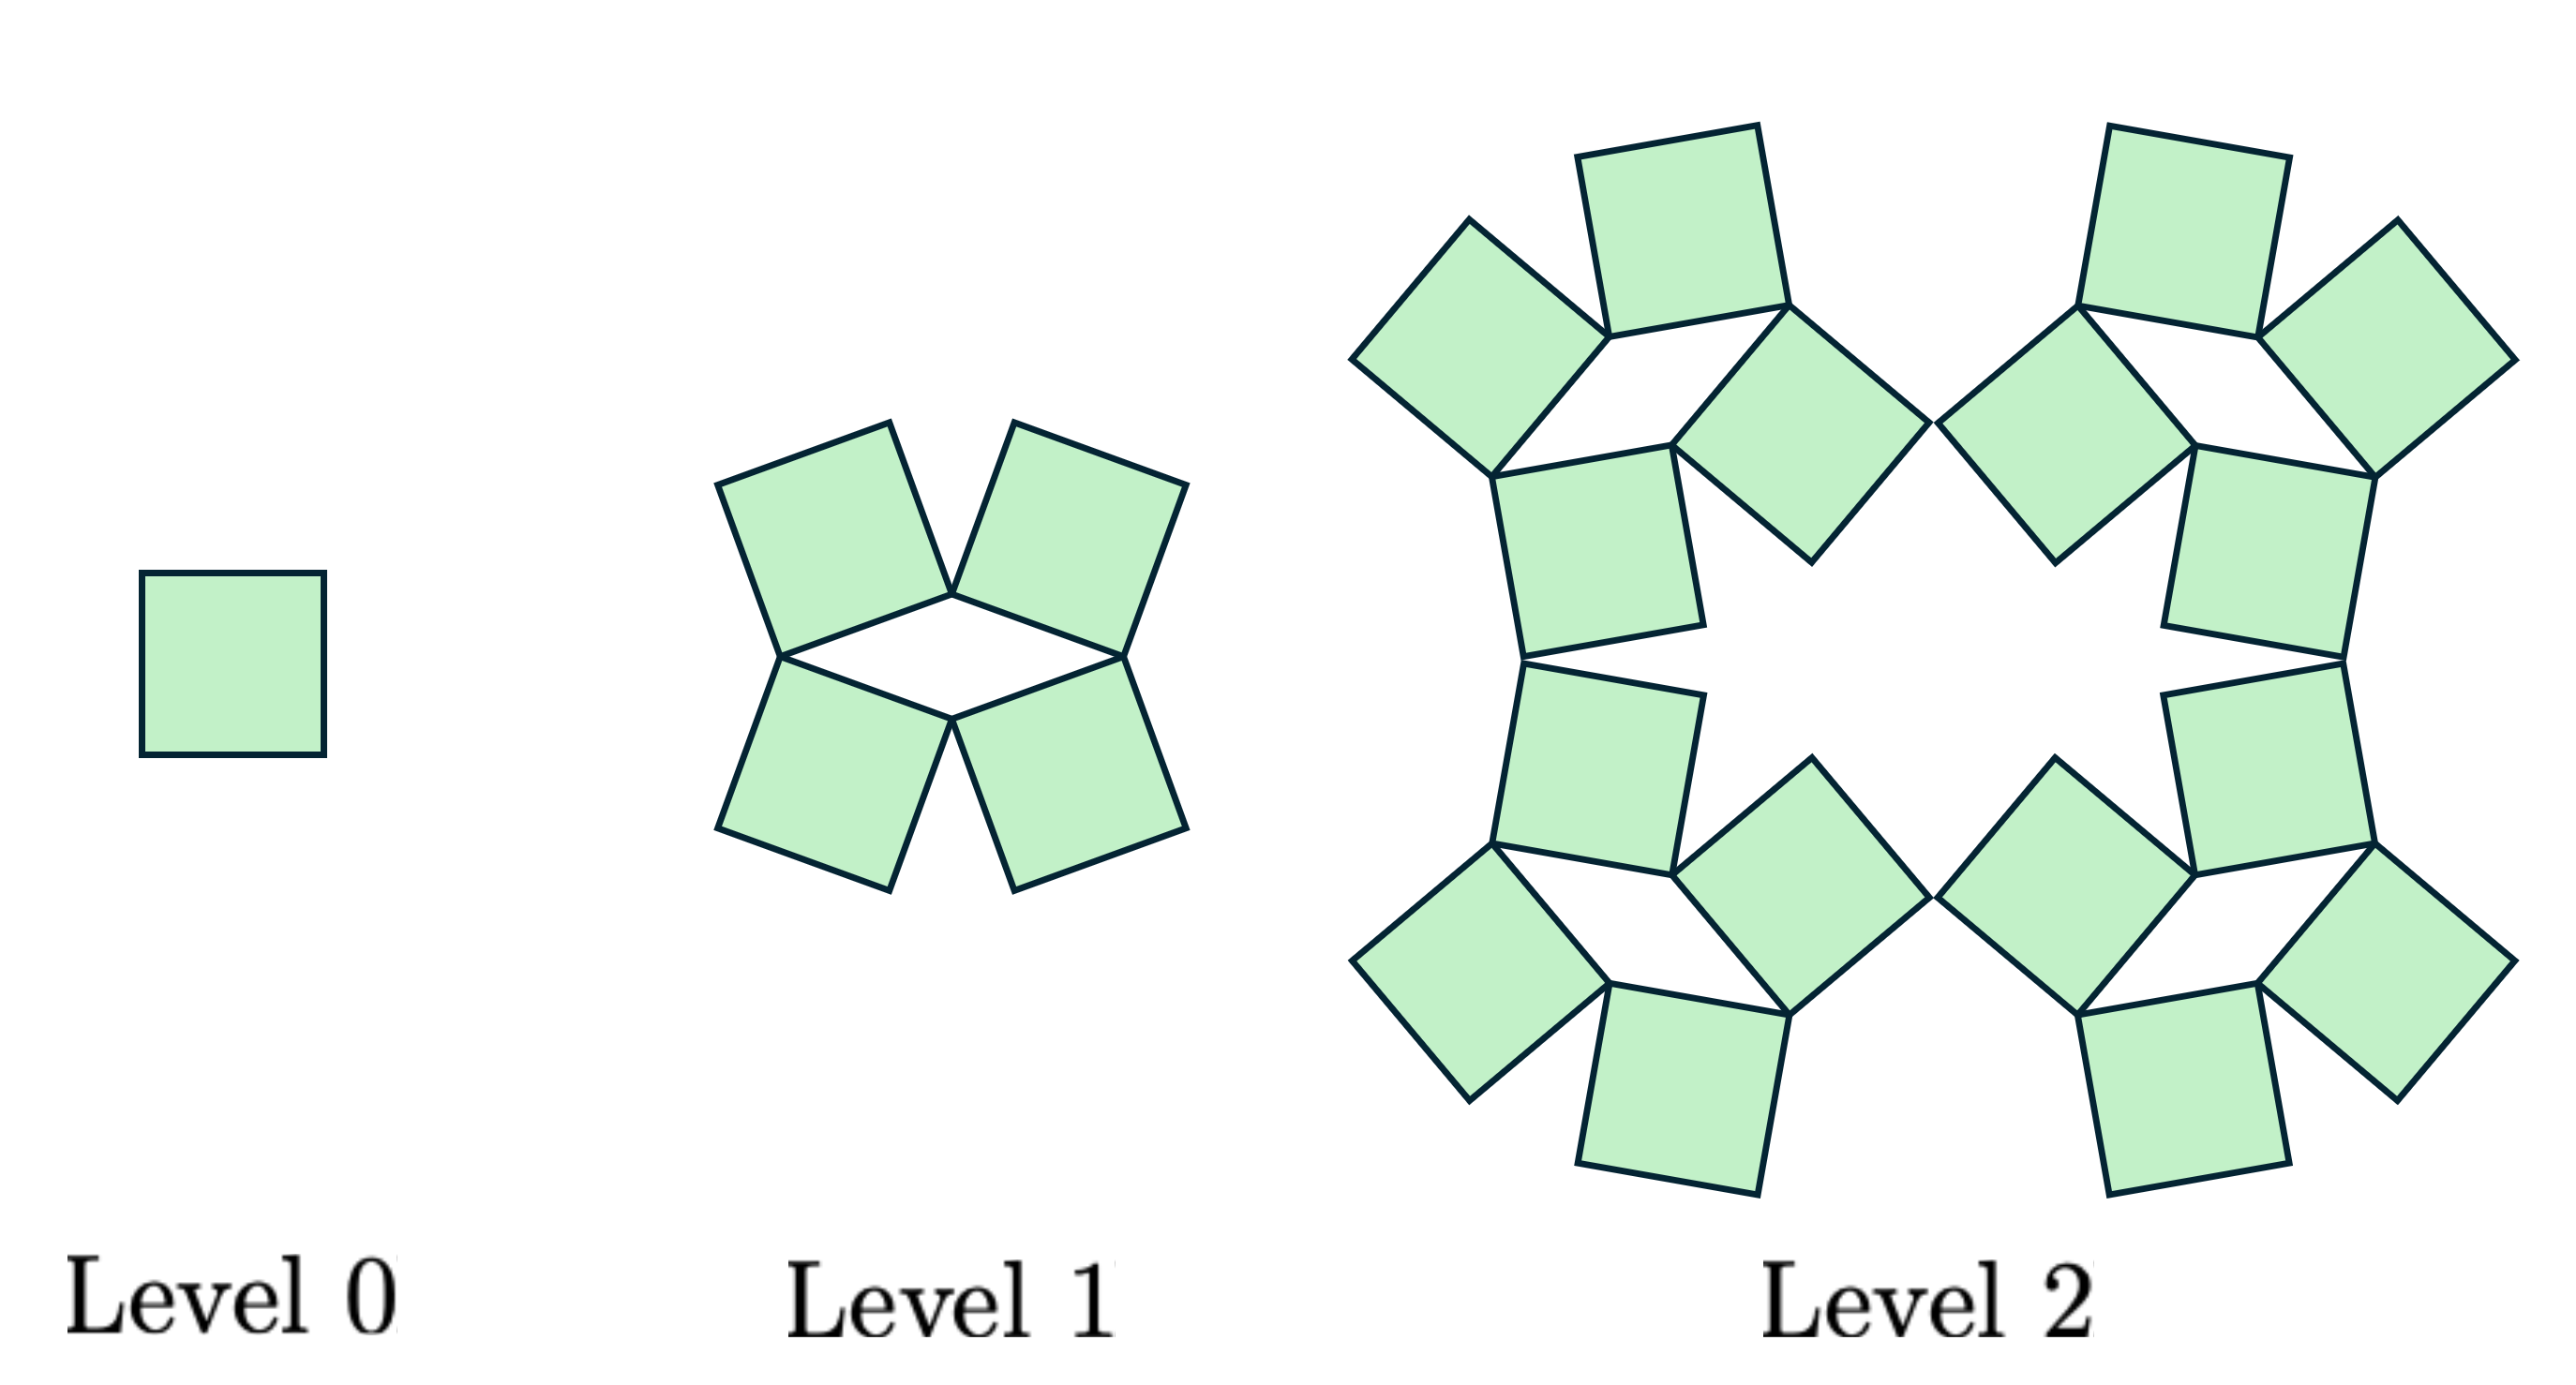
\includegraphics[width=0.45\textwidth]{figures/fractal1.png}
  \caption{Construcción jerárquica de la estructura. El nivel 0
  corresponde a un cuadrado elemental; los niveles 1 y 2 se obtienen
  ensamblando cuatro copias del nivel anterior. Las conexiones
  permiten la rotación relativa de las unidades.}
  \label{fig:levels}
\end{figure}

\paragraph{Ángulos de las bisagras.}

En cada nivel distinguimos dos familias de bisagras, asociadas a los
ángulos $\phi_i^+$ y $\phi_i^-$ de la Fig.~\ref{fig:angles}. Estos
ángulos combinan la rotación propia del nivel con las rotaciones
acumuladas de los niveles que lo componen:
\begin{equation}
\phi_i^+ = \pi-(\theta_i+S_i),
\qquad
\phi_i^- = \theta_i-S_i,
\label{eq:phi_combined}
\end{equation}
donde
\begin{equation}
S_i=\sum_{j=1}^{i-1}\theta_j,
\qquad S_1=0.
\label{eq:Si_def}
\end{equation}
Los índices aumentan desde las escalas más pequeñas hacia las más
grandes. Por ello, $S_i$ recoge las contribuciones de los niveles
internos $j<i$ a los ángulos de las bisagras del nivel $i$.

\begin{figure}[H]
  \centering
  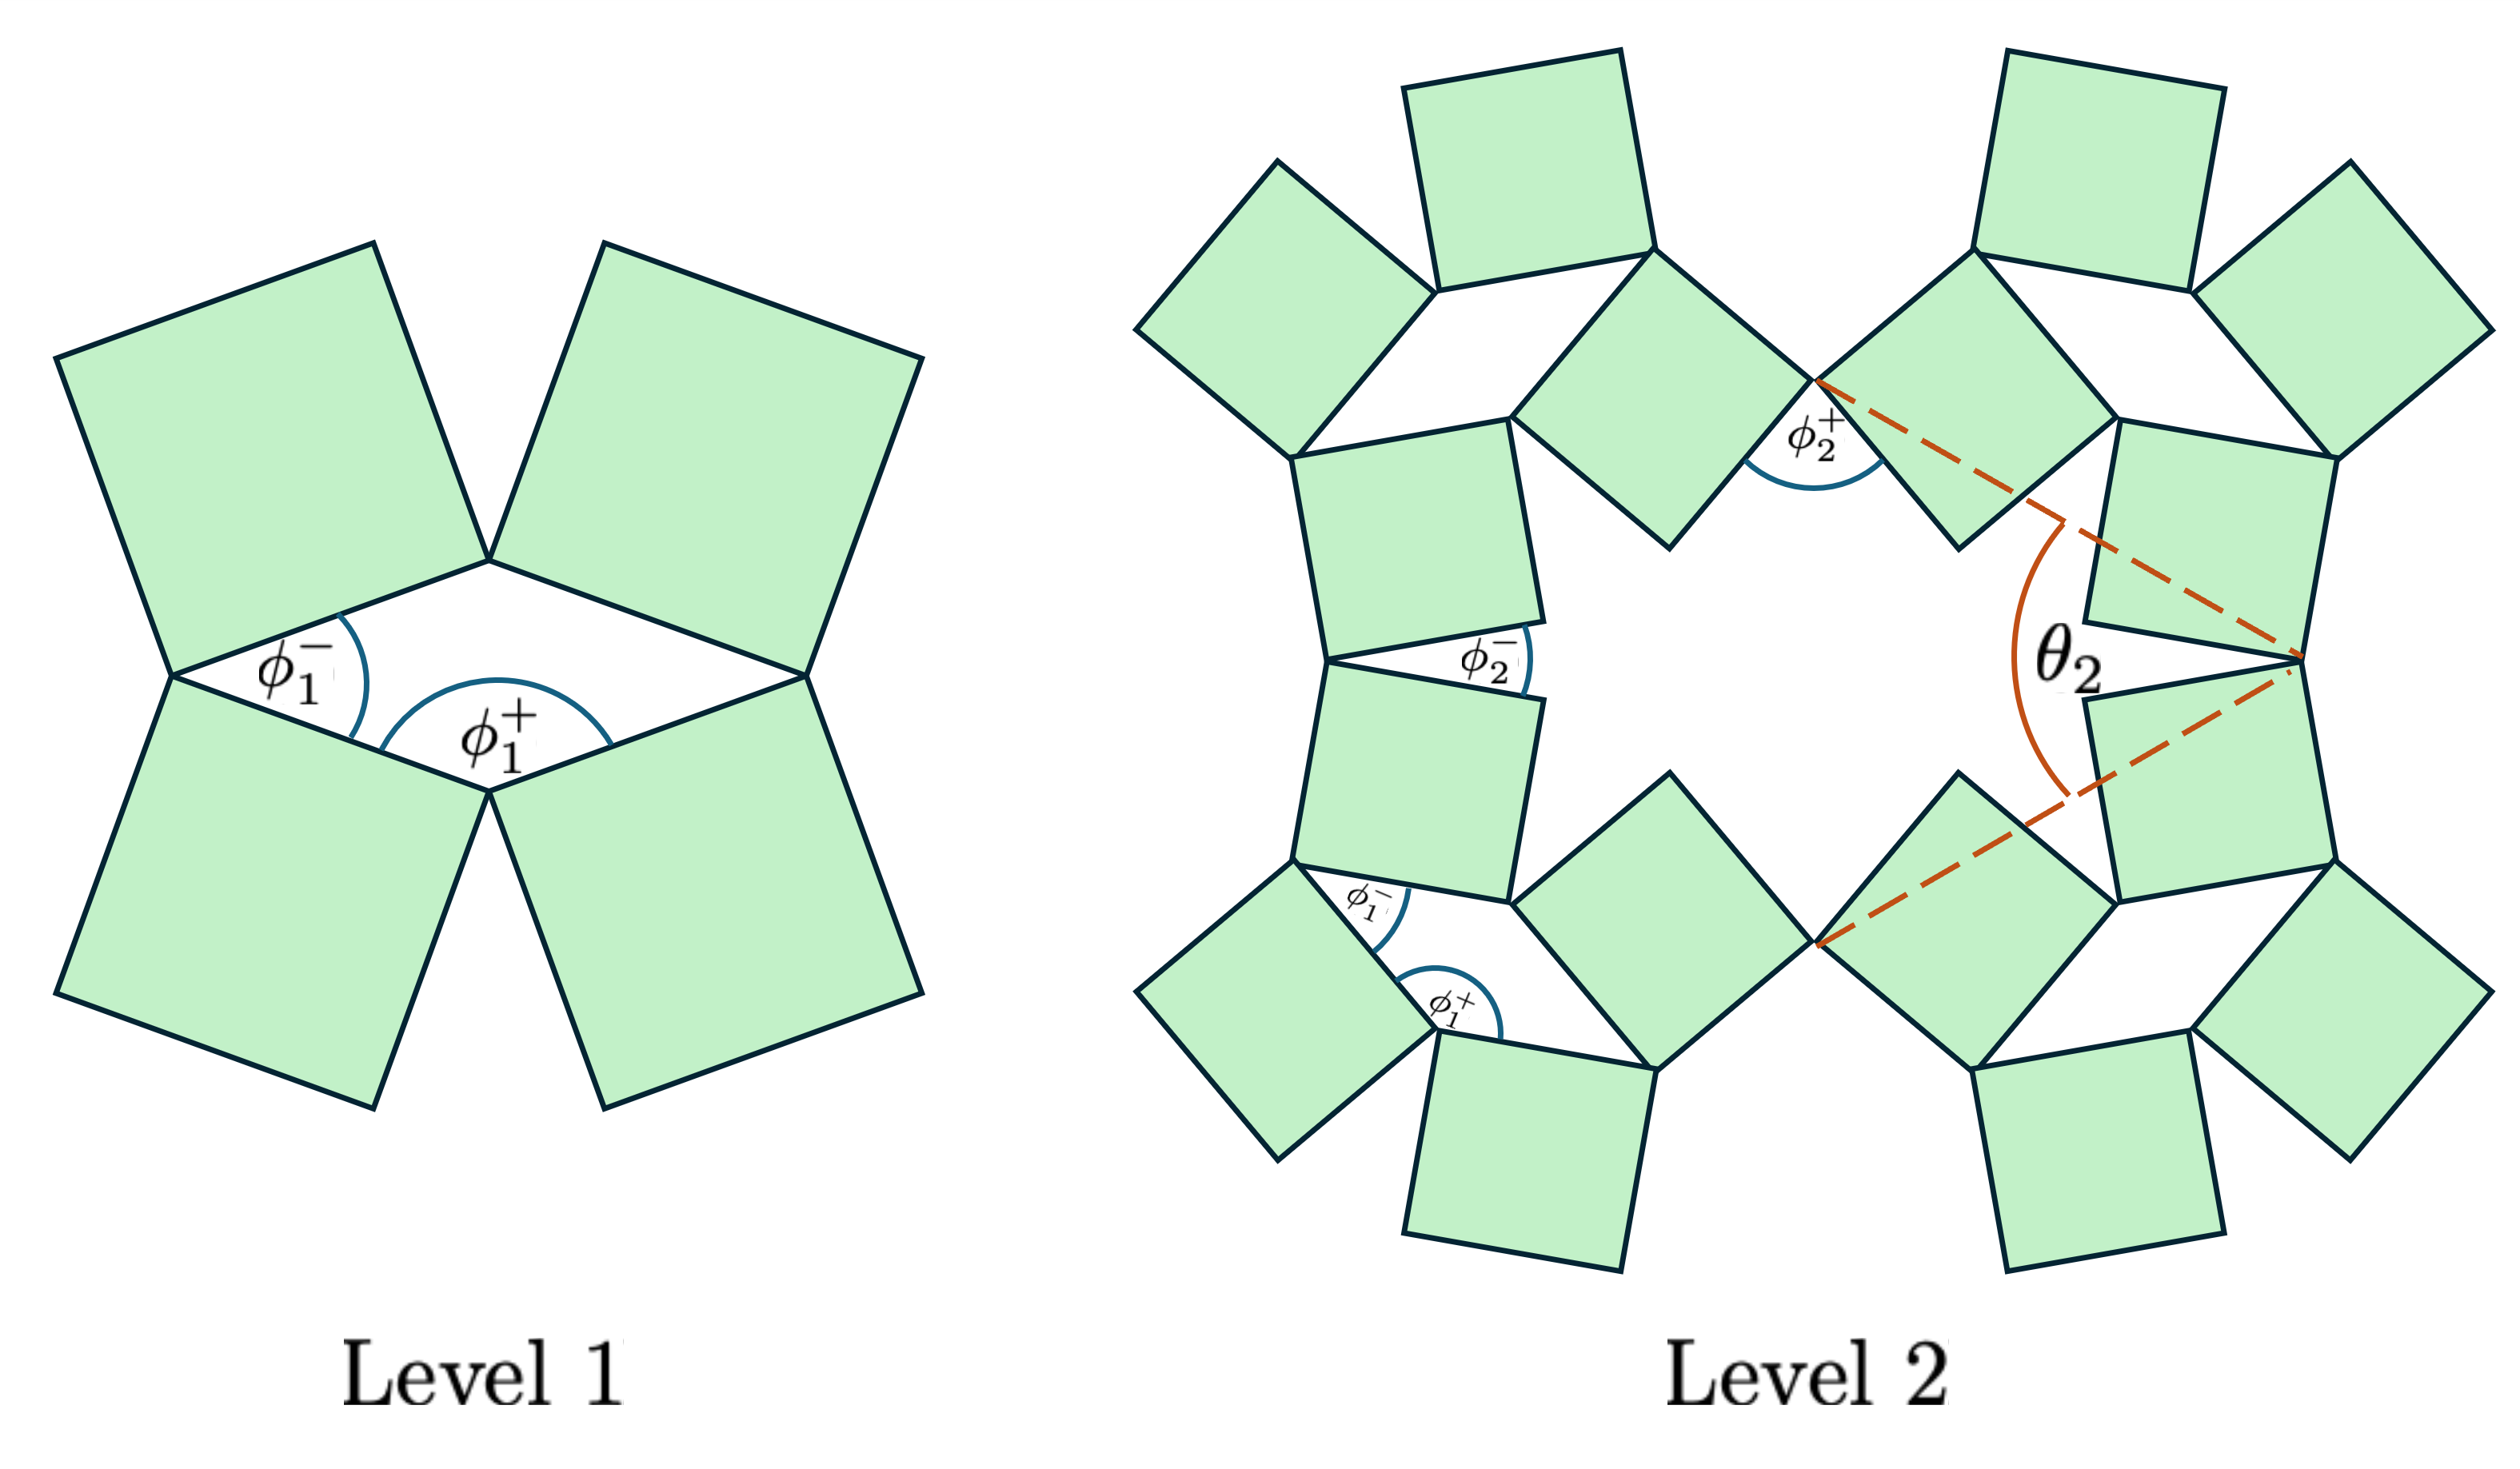
\includegraphics[width=0.45\textwidth]{figures/fractal2.png}
  \caption{Definición de las dos familias de ángulos de bisagra,
  $\phi_i^+$ y $\phi_i^-$, y su relación con las rotaciones
  elementales $\theta_i$. Las rotaciones de los niveles internos
  contribuyen mediante la suma acumulada $S_i$.}
  \label{fig:angles}
\end{figure}

\paragraph{Configuración natural de las bisagras.}

La estructura no tiene por qué estar relajada en
$\theta_i=0$. Denotamos por
\begin{equation}
\boldsymbol{\theta}^{(0)}
=
(\theta_1^{(0)},\ldots,\theta_N^{(0)})
\label{eq:theta_rest_def}
\end{equation}
su configuración natural, es decir, la geometría en ausencia de
carga externa. Esta elección determina también, y no de manera
independiente, los ángulos naturales de ambas familias de bisagras.
Definiendo
\begin{equation}
S_i^{(0)}=\sum_{j=1}^{i-1}\theta_j^{(0)},
\qquad S_1^{(0)}=0,
\label{eq:Si_rest_def}
\end{equation}
se tiene
\begin{equation}
\phi_{i,0}^{+}
=\pi-\left(\theta_i^{(0)}+S_i^{(0)}\right),
\qquad
\phi_{i,0}^{-}
=\theta_i^{(0)}-S_i^{(0)}.
\label{eq:phi_rest_def}
\end{equation}
Por construcción, una misma configuración
$\boldsymbol{\theta}^{(0)}$ es compatible simultáneamente con
$\phi_{i,0}^{+}$ y $\phi_{i,0}^{-}$. En particular, permitir
$\boldsymbol{\theta}^{(0)}\neq\boldsymbol{0}$ introduce una
deformación geométrica inicial sin generar tensiones residuales:
la energía elástica sigue siendo nula en
$\boldsymbol{\theta}=\boldsymbol{\theta}^{(0)}$.

\paragraph{Energía elástica.}

Las dos familias de bisagras se distinguen por su dependencia
geométrica con los ángulos $\theta_i$, pero comparten una única
constante elástica $k_i>0$ en cada nivel. Ambas familias contribuyen
simultáneamente a la energía, con la misma rigidez.

La contribución elástica de una unidad del nivel $i$ se escribe como
\begin{equation}
E^{(i)}
=2k_i\left[
\left(\phi_i^--\phi_{i,0}^-\right)^2
+
\left(\phi_i^+-\phi_{i,0}^+\right)^2
\right].
\label{eq:Ei_phi}
\end{equation}
Al sustituir las Ecs.~\eqref{eq:phi_combined} y
\eqref{eq:phi_rest_def} y sumar todos los niveles con su
multiplicidad geométrica, se obtiene la energía total:
\begin{equation}
\boxed{
\begin{aligned}
E_N(\boldsymbol{\theta};\boldsymbol{\theta}^{(0)})
={}&2\sum_{i=1}^{N}4^{N-i}k_i
\Bigg\{
\left[
(\theta_i-S_i)-(\theta_i^{(0)}-S_i^{(0)})
\right]^2
\\[-0.2em]
&\qquad+
\left[
(\theta_i+S_i)-(\theta_i^{(0)}+S_i^{(0)})
\right]^2
\Bigg\}.
\end{aligned}
}
\label{eq:En_theta_final}
\end{equation}
Esta expresión separa claramente tres ingredientes: la multiplicidad
jerárquica $4^{N-i}$, la rigidez $k_i$ y la geometría natural
$\boldsymbol{\theta}^{(0)}$. Para evitar operar numéricamente con
factores muy grandes y rigideces muy pequeñas, también puede
introducirse el peso efectivo
\begin{equation}
w_i\equiv 2\,4^{N-i}k_i,
\label{eq:effective_weight}
\end{equation}
de modo que la energía es simplemente la suma de $w_i$ multiplicado
por los dos residuos cuadráticos de la Ec.~\eqref{eq:En_theta_final}.

% =================================================
\section{Tamaños del sistema}
\label{sec:size}
% =================================================

La geometría de la estructura se caracteriza mediante las cuatro
distancias indicadas en la Fig.~\ref{fig:size}, que denotamos por
$Lx_{\max}$, $Lx_{\min}$, $Ly_{\max}$ y $Ly_{\min}$.
Estas cantidades se calculan de forma recursiva a partir de los
ángulos $\{\theta_i\}$.

Elegimos como unidad de longitud la extensión horizontal de la
estructura con todos sus ángulos nulos. Para una jerarquía de
$N$ niveles, el lado del cuadrado elemental es entonces $2^{-N}$.
Los valores de partida de la construcción geométrica son
\begin{equation}
Lx_{\max}^{(0)}=Lx_{\min}^{(0)}
=Ly_{\max}^{(0)}=Ly_{\min}^{(0)}=2^{-N}.
\label{eq:size_base}
\end{equation}
Con esta normalización,
$Lx_{\max}^{(N)}=Ly_{\max}^{(N)}=1$
cuando $\theta_i=0$ para todos los niveles. Esta elección fija
únicamente la unidad de longitud: la longitud inicial $L_0$ se
calcula en la configuración natural $\boldsymbol{\theta}^{(0)}$
y, en general, no es igual a uno.

\begin{figure}[H]
  \centering
  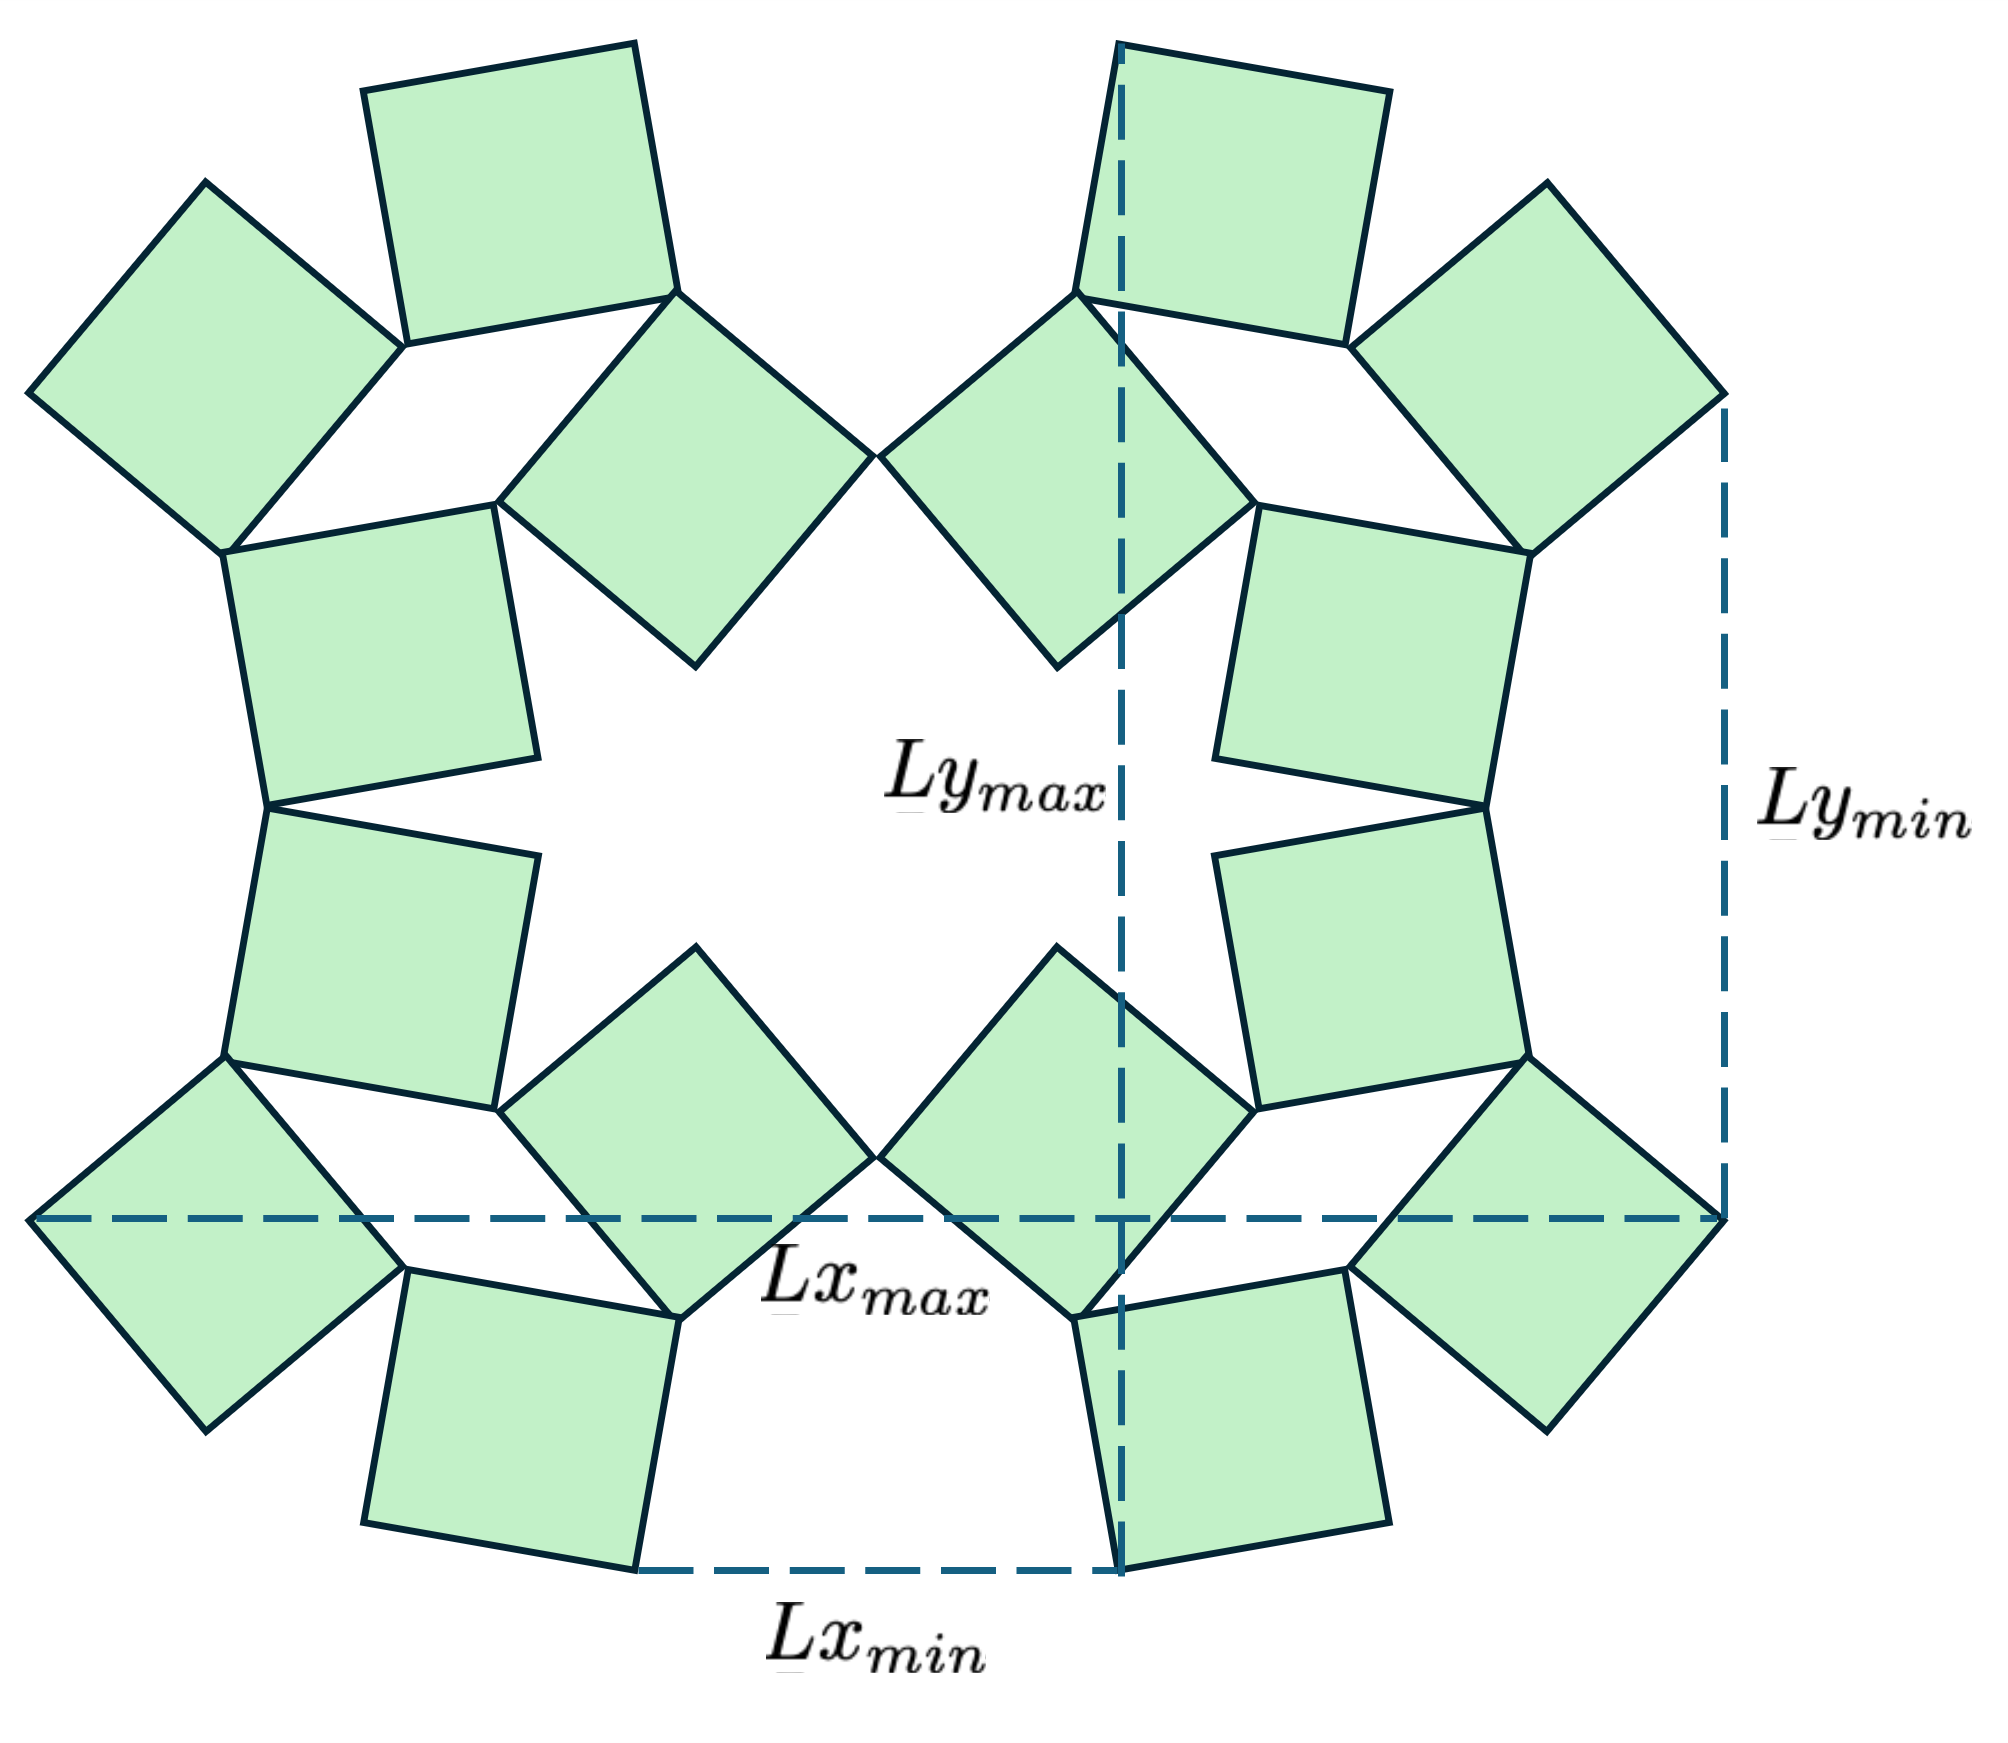
\includegraphics[width=0.45\textwidth]{figures/fractal3.png}
  \caption{Distancias características de la estructura en las
  direcciones horizontal y vertical. Estas magnitudes se obtienen
  mediante la construcción geométrica recursiva.}
  \label{fig:size}
\end{figure}

Al ensamblar cuatro unidades del nivel $i-1$, sus dimensiones se
proyectan sobre los ejes horizontal y vertical mediante los factores
$\sin(\theta_i/2)$ y $\cos(\theta_i/2)$.
Para la geometría representada en la Fig.~\ref{fig:size}, se obtienen
las recurrencias
\begin{align}
Ly_{\max}^{(i)}
&=
2\sin\!\left(\frac{\theta_i}{2}\right)Lx_{\max}^{(i-1)}
+
2\cos\!\left(\frac{\theta_i}{2}\right)Ly_{\min}^{(i-1)},
\label{eq:Lymax_rec}
\\
Lx_{\min}^{(i)}
&=
2\sin\!\left(\frac{\theta_i}{2}\right)Ly_{\min}^{(i-1)},
\label{eq:Lxmin_rec}
\\
Lx_{\max}^{(i)}
&=
2\cos\!\left(\frac{\theta_i}{2}\right)Lx_{\max}^{(i-1)}
+
2\sin\!\left(\frac{\theta_i}{2}\right)Ly_{\min}^{(i-1)},
\label{eq:Lxmax_rec}
\\
Ly_{\min}^{(i)}
&=
2\cos\!\left(\frac{\theta_i}{2}\right)Ly_{\min}^{(i-1)}.
\label{eq:Lymin_rec}
\end{align}
En cada paso, todas las cantidades del lado derecho corresponden
al nivel anterior.

Estas relaciones dependen únicamente de la configuración angular.
Las rigideces y la configuración natural intervienen en las
longitudes de equilibrio a través de los ángulos seleccionados
por la energía elástica.

La recurrencia para $Ly_{\min}^{(i)}$ puede resolverse directamente:
\begin{equation}
Ly_{\min}^{(i)}
=
2^{i-N}
\prod_{j=1}^{i}
\cos\!\left(\frac{\theta_j}{2}\right).
\label{eq:Lymin_product}
\end{equation}
Al sustituir esta expresión en la recurrencia de
$Lx_{\max}^{(i)}$ e iterar hasta el nivel $N$, resulta
\begin{equation}
\boxed{
Lx_{\max}^{(N)}
=
\prod_{i=1}^{N}\cos\!\left(\frac{\theta_i}{2}\right)
+
\sum_{i=1}^{N}
\left[
\sin\!\left(\frac{\theta_i}{2}\right)
\prod_{\substack{j=1\\j\neq i}}^{N}
\cos\!\left(\frac{\theta_j}{2}\right)
\right].
}
\label{eq:Lxmax_product}
\end{equation}
Esta forma es válida también cuando alguno de los cosenos se anula.
Cuando todos son distintos de cero, puede escribirse equivalentemente
como
\begin{equation}
Lx_{\max}^{(N)}
=
\left[
\prod_{i=1}^{N}\cos\!\left(\frac{\theta_i}{2}\right)
\right]
\left[
1+\sum_{i=1}^{N}\tan\!\left(\frac{\theta_i}{2}\right)
\right].
\label{eq:Lxmax_factored}
\end{equation}
Ambas expresiones conservan la dependencia trigonométrica completa
de la construcción recursiva, sin introducir una aproximación de
pequeños ángulos.

\subsection{Deformación y extensión máxima}
\label{sec:strain_max}

La longitud inicial se define a partir de la misma configuración
natural que fija los ángulos de reposo de las bisagras:
\begin{equation}
L_0\equiv Lx_{\max}^{(N)}(\boldsymbol{\theta}^{(0)})>0.
\label{eq:L0_general}
\end{equation}
La Ec.~\eqref{eq:Lxmax_product} permite calcularla para cualquier
configuración inicial admisible. Definimos entonces
\begin{equation}
\boxed{
\varepsilon(\boldsymbol{\theta};\boldsymbol{\theta}^{(0)})
=\frac{Lx_{\max}^{(N)}(\boldsymbol{\theta})-L_0}{L_0}.
}
\label{eq:strain_def}
\end{equation}
Así, $\varepsilon=0$ en la configuración natural; los valores
positivos y negativos corresponden, respectivamente, a extensión
y compresión respecto de ella. La relación
$\varepsilon=Lx_{\max}^{(N)}-1$ se recupera cuando
$\boldsymbol{\theta}^{(0)}=\boldsymbol{0}$.

Para ángulos actuales e iniciales pequeños y un número fijo de
niveles, la expansión hasta segundo orden da
\begin{equation}
\varepsilon
=
\frac{
\frac12\sum_{i=1}^{N}(\theta_i-\theta_i^{(0)})
-\frac18\sum_{i=1}^{N}\left[\theta_i^2-(\theta_i^{(0)})^2\right]
}{
1+\frac12\sum_{i=1}^{N}\theta_i^{(0)}
-\frac18\sum_{i=1}^{N}(\theta_i^{(0)})^2
}
+O(\eta^3),
\label{eq:strain_small_angles}
\end{equation}
donde $\eta=\max_i\{|\theta_i|,|\theta_i^{(0)}|\}$.
Esta aproximación no es uniforme al aumentar $N$; para analizar
ese límite conservamos la expresión trigonométrica completa.

Para determinar la extensión máxima y su dependencia con $N$,
consideramos la expresión geométrica completa. Denotamos por
$X_N^\star$ el máximo de $Lx_{\max}^{(N)}$ respecto de los
ángulos de apertura en la rama $0\leq\theta_i\leq\pi$, dentro
de la cinemática reducida y sin restricciones adicionales de contacto.

La maximización conduce a una configuración en la que todos
los ángulos son iguales,
\begin{equation}
\theta_i=\theta_N^\star,
\qquad i=1,\ldots,N.
\end{equation}
Para un ángulo común $\theta$, la longitud se escribe como
\begin{equation}
X_N(\theta)
=
\cos^N\!\left(\frac{\theta}{2}\right)
\left[
1+N\tan\!\left(\frac{\theta}{2}\right)
\right].
\label{eq:length_equal_angles}
\end{equation}

Introduciendo $t=\tan(\theta/2)$, resulta
\begin{equation}
X_N(t)=\frac{1+Nt}{(1+t^2)^{N/2}}.
\end{equation}
La condición de máximo,
$\mathrm{d}X_N/\mathrm{d}t=0$, implica
\begin{equation}
(N-1)t^2+t-1=0.
\end{equation}
Su solución positiva es
\begin{equation}
t_N^\star
=
\frac{2}{1+\sqrt{4N-3}},
\qquad
\theta_N^\star=2\arctan(t_N^\star).
\label{eq:theta_max_extension}
\end{equation}
Por tanto, la longitud y la deformación máximas son
\begin{equation}
X_N^\star
=
\frac{1+Nt_N^\star}
{\left[1+(t_N^\star)^2\right]^{N/2}},
\qquad
\varepsilon_{\max}=\frac{X_N^\star}{L_0}-1.
\label{eq:max_extension_finite_N}
\end{equation}

En el límite de muchos niveles,
\begin{equation}
t_N^\star\sim N^{-1/2},
\qquad
\theta_N^\star\sim\frac{2}{\sqrt{N}}.
\end{equation}
En consecuencia,
\begin{equation}
1+Nt_N^\star\sim\sqrt{N},
\qquad
\left[1+(t_N^\star)^2\right]^{-N/2}
\longrightarrow e^{-1/2},
\end{equation}
y obtenemos
\begin{equation}
\boxed{
X_N^\star\sim\sqrt{\frac{N}{e}},
\qquad N\to\infty.
}
\label{eq:max_extension_scaling}
\end{equation}

Así, la longitud máxima crece como $\sqrt{N}$, mientras que
la rotación correspondiente disminuye como $N^{-1/2}$. El
comportamiento de $\varepsilon_{\max}$ depende además de cómo
varía $L_0$ con $N$. Para la configuración inicial nula,
$L_0=1$ y se recupera $\varepsilon_{\max}\sim\sqrt{N/e}$.

\subsection{Configuración inicial proporcional al ángulo de máxima extensión}
\label{sec:initial_fraction}

Consideramos ahora una configuración natural uniforme,
\begin{equation}
\theta_i^{(0)}=c\,\theta_N^\star,
\qquad i=1,\ldots,N,\qquad 0\leq c\leq1,
\label{eq:theta_initial_fraction}
\end{equation}
donde $c$ es una constante independiente de $N$. Este intervalo
sitúa el estado inicial en la rama de longitud creciente de la
familia de ángulos iguales. Los ángulos naturales $\phi_{i,0}^{\pm}$
quedan determinados por la Ec.~\eqref{eq:phi_rest_def}.
La longitud inicial y la deformación máxima son entonces
\begin{align}
L_0(N,c)
&=X_N(c\,\theta_N^\star)
=\cos^N\!\left(\frac{c\,\theta_N^\star}{2}\right)
\left[1+N\tan\!\left(\frac{c\,\theta_N^\star}{2}\right)\right],
\label{eq:L0_fraction}
\\
\varepsilon_{\max}(N,c)
&=\frac{X_N^\star}{X_N(c\,\theta_N^\star)}-1.
\label{eq:strain_max_fraction}
\end{align}

Para describir geométricamente la extensión desde ese estado,
podemos recorrer las configuraciones uniformes
$\theta_i=u\,\theta_N^\star$, con $c\leq u\leq1$. Sobre esta familia,
\begin{equation}
\varepsilon_N(u;c)
=\frac{X_N(u\,\theta_N^\star)}{X_N(c\,\theta_N^\star)}-1,
\label{eq:strain_uniform_path}
\end{equation}
que crece desde cero en $u=c$ hasta $\varepsilon_{\max}(N,c)$
en $u=1$. Esta parametrización describe una familia geométrica;
la trayectoria de equilibrio bajo carga debe determinarse a partir
de la energía y no tiene por qué mantener todos los ángulos iguales.

Para $0<c\leq1$ fijo y $N\to\infty$, se obtiene
\begin{equation}
L_0(N,c)\sim c\,e^{-c^2/2}\sqrt{N},
\qquad
\boxed{
\varepsilon_{\max}(N,c)
\longrightarrow \frac{e^{(c^2-1)/2}}{c}-1.
}
\label{eq:strain_max_fraction_limit}
\end{equation}
Más generalmente, para $c\leq u\leq1$,
\begin{equation}
\varepsilon_N(u;c)
\longrightarrow
\frac{u}{c}\exp\!\left(\frac{c^2-u^2}{2}\right)-1.
\label{eq:strain_uniform_limit}
\end{equation}
Por tanto, una fracción inicial $0<c<1$ produce una capacidad de
extensión relativa que tiende a un valor finito y positivo, aunque
las longitudes inicial y máxima crecen ambas como $\sqrt{N}$.
Aumentar $c$ reduce esa capacidad; para $c=1$, la estructura parte
de su longitud máxima y $\varepsilon_{\max}=0$. El caso $c=0$
debe tratarse por separado: $L_0=1$ y la deformación máxima crece
como $\sqrt{N/e}$. El límite anterior no es uniforme cerca de $c=0$.

Aunque los ángulos iniciales tienden a cero para $c$ fijo,
$\sum_i(\theta_i^{(0)})^2\to4c^2$ y, en la configuración de
máxima extensión, $\sum_i(\theta_N^\star)^2\to4$. Por ello,
la expansión~\eqref{eq:strain_small_angles} no basta para obtener
estos límites: debe conservarse el efecto acumulado del producto
de cosenos.

La extensión máxima caracteriza una capacidad geométrica.
La trayectoria de equilibrio y la fuerza necesaria para aproximarse
a ella dependen de las rigideces $\{k_i\}$ y de la configuración
natural $\boldsymbol{\theta}^{(0)}$.

% =================================================
\section{Hamiltoniano a longitud impuesta: caso $w_i=1$}
\label{sec:hamiltonian}
% =================================================

En lo que sigue consideramos pesos efectivos uniformes. Con la
convención de la Ec.~\eqref{eq:effective_weight}, esto significa
\begin{equation}
w_i=2\,4^{N-i}k_i=1,
\qquad k_i=\frac12\,4^{i-N}.
\label{eq:uniform_weights}
\end{equation}
Esta elección compensa la multiplicidad geométrica de cada nivel;
las dos familias de bisagras conservan la misma rigidez $k_i$.
Estudiamos la rama de tracción conectada al reposo, con $f\geq0$,
y tomamos $N\geq2$ y $\theta_i^{(0)}=c\,\theta_N^\star$,
con $0<c<1$ fijo al variar $N$.

\subsection{Energía y restricción geométrica}

Definimos los desplazamientos angulares y sus sumas acumuladas por
\begin{equation}
\delta_i=\theta_i-\theta_i^{(0)},
\qquad D_i=\sum_{j<i}\delta_j.
\end{equation}
Al sumar las contribuciones de ambas familias, los términos cruzados
se cancelan y la energía toma la forma exacta
\begin{equation}
\boxed{
E_N=\sum_{i=1}^{N}\left[(\delta_i-D_i)^2+(\delta_i+D_i)^2\right]
=2\sum_{i=1}^{N}(\delta_i^2+D_i^2).
}
\label{eq:uniform_energy_matrix}
\end{equation}
Introduciendo la matriz de sumas acumuladas
\begin{equation}
T_{ij}=\begin{cases}1,&j<i,\\0,&j\geq i,\end{cases}
\qquad K=4(I+T^{\mathsf T}T),
\label{eq:K_uniform}
\end{equation}
se obtiene $E_N=\tfrac12\boldsymbol\delta^{\mathsf T}K\boldsymbol\delta$.
La matriz $K$ es definida positiva y no depende de la configuración
natural; esta última interviene en la geometría de la respuesta.

Denotamos la longitud horizontal por
\begin{equation}
X(\boldsymbol\theta)\equiv Lx_{\max}^{(N)}(\boldsymbol\theta),
\qquad L_0=X(\boldsymbol\theta^{(0)}).
\label{eq:X_def}
\end{equation}
Al imponer una longitud $\ell$, la deformación prescrita es
$\varepsilon=(\ell-L_0)/L_0$. Introducimos el Hamiltoniano restringido
\begin{equation}
\boxed{
\mathcal H(\boldsymbol\theta,f;\ell)
=\frac12\boldsymbol\delta^{\mathsf T}K\boldsymbol\delta
-f\left[X(\boldsymbol\theta)-\ell\right],
\qquad \ell=L_0(1+\varepsilon).
}
\label{eq:H_def_ki}
\end{equation}
Aquí $f$ es el multiplicador de Lagrange conjugado a la longitud
normalizada. A longitud impuesta, tanto $f$ como los ángulos son
incógnitas. Las condiciones de equilibrio son
\begin{equation}
\boxed{
K\boldsymbol\delta=f\,\nabla X(\boldsymbol\theta),
\qquad X(\boldsymbol\theta)=\ell.
}
\label{eq:equilibrium_general}
\end{equation}
El equilibrio estable corresponde a un mínimo de la energía bajo
la restricción. En un punto regular, donde $\nabla X\neq0$, una
condición necesaria es que $K-f\nabla^2X$ sea semidefinida positiva
sobre las variaciones $\mathbf v$ que satisfacen
$\nabla X^{\mathsf T}\mathbf v=0$; la positividad estricta sobre
ese espacio es suficiente para un mínimo local estricto.
Las ecuaciones anteriores conservan la geometría trigonométrica
completa. Puede parametrizarse la rama mediante $f$ y calcular
$\ell=X(\boldsymbol\theta(f))$; a longitud impuesta se selecciona
el valor de $f$ que satisface la restricción.

% =================================================
\section{Respuesta alrededor de la configuración natural}
\label{sec:small}
% =================================================

Desarrollamos la geometría en los desplazamientos respecto de
$\boldsymbol\theta^{(0)}$.
Definimos
\begin{equation}
\mathbf g=\nabla X\big|_{\boldsymbol\theta^{(0)}},
\qquad Q=-\nabla^2X\big|_{\boldsymbol\theta^{(0)}}.
\end{equation}
Para $N$ fijo, la expansión de la longitud es
\begin{equation}
X(\boldsymbol\theta^{(0)}+\boldsymbol\delta)
=L_0+\mathbf g^{\mathsf T}\boldsymbol\delta
-\frac12\boldsymbol\delta^{\mathsf T}Q\boldsymbol\delta
+O(\|\boldsymbol\delta\|^3).
\label{eq:X_local}
\end{equation}
Esta expansión mantiene la dependencia exacta de sus coeficientes
con los ángulos iniciales.

\subsection{Coeficientes geométricos para el reposo uniforme}

Sea $t_0=\tan(c\theta_N^\star/2)$ y
$P_0=\cos^N(c\theta_N^\star/2)$. Por la simetría de la longitud,
\begin{equation}
L_0=P_0(1+Nt_0),\qquad
\mathbf g=g\mathbf1,\qquad Q=aI+b\mathbf1\mathbf1^{\mathsf T},
\label{eq:uniform_geometry_coefficients}
\end{equation}
donde $\mathbf1$ es el vector de componentes unitarias y
\begin{align}
g&=\frac{P_0}{2}\left[1-t_0-(N-1)t_0^2\right],\\
b&=\frac{P_0}{4}\left[2t_0-t_0^2-(N-2)t_0^3\right],\\
a&=\frac{L_0}{4}-b.
\label{eq:gab_def}
\end{align}
Para $N\geq2$ y $0<c<1$, estos coeficientes son positivos.
En el límite de muchos niveles, con $c$ fijo,
\begin{equation}
\begin{aligned}
L_0&\sim c e^{-c^2/2}\sqrt N,
& g&\sim\frac{1-c^2}{2}e^{-c^2/2},\\
a&\sim\frac{c}{4}e^{-c^2/2}\sqrt N,
& b&\sim\frac{c(2-c^2)}{4\sqrt N}e^{-c^2/2}.
\end{aligned}
\label{eq:geometry_coefficients_scaling}
\end{equation}

\subsection{Régimen hookeano}

A primer orden en la carga, las ecuaciones de equilibrio dan
$\boldsymbol\delta=fK^{-1}\mathbf g+O(f^2)$. Por tanto,
\begin{equation}
\boxed{
\varepsilon=\chi_0 f+O(f^2),\qquad
\chi_0=\frac{g^2}{L_0}h_N(0).
}
\label{eq:hookean_compliance}
\end{equation}
Aquí hemos introducido, para $q\geq0$, la función
\begin{equation}
h_N(q)=\mathbf1^{\mathsf T}(K+qI)^{-1}\mathbf1,
\label{eq:resolvent_definition}
\end{equation}
que recoge la respuesta angular a una carga uniforme.
La rigidez inicial respecto de la deformación relativa es
$K_{\mathrm{eff}}=(\mathrm df/\mathrm d\varepsilon)_{f=0}=\chi_0^{-1}$;
respecto de la elongación absoluta es
$(\mathrm df/\mathrm d\ell)_{\ell=L_0}=(g^2h_N(0))^{-1}$.

Para calcular $h_N$, sea $\mathbf v=(K+qI)^{-1}\mathbf1$ y
$s_j=\sum_{i=1}^{j}v_i$, con $s_0=0$. Escribiendo $d=4+q$,
las ecuaciones se reducen a
\begin{equation}
d(2s_j-s_{j-1}-s_{j+1})+4s_j=0\quad(1\leq j<N),
\qquad d(s_N-s_{N-1})=1.
\end{equation}
Su solución proporciona
\begin{equation}
\boxed{
h_N(q)=\frac{\sinh(N\kappa)}
{d[\sinh(N\kappa)-\sinh((N-1)\kappa)]},
\qquad \cosh\kappa=1+\frac{2}{d}.
}
\label{eq:resolvent_exact}
\end{equation}
En particular, $h_N(0)\to(1+\sqrt5)/8$. Así,
\begin{equation}
\chi_0\sim
\frac{(1+\sqrt5)(1-c^2)^2e^{-c^2/2}}{32c\sqrt N},
\qquad K_{\mathrm{eff}}\propto\sqrt N.
\label{eq:hookean_scaling}
\end{equation}
Para cada tamaño finito existe, por tanto, una respuesta hookeana
cerca del reposo. Su intervalo de validez puede disminuir al
incrementar $N$.

% =================================================
\section{Cruce hacia la respuesta no hookeana}
\label{sec:crossover}
% =================================================

\subsection{Solución con la curvatura geométrica}

Al conservar el término cuadrático de la longitud, el equilibrio
del modelo local satisface
\begin{equation}
(K+fQ)\boldsymbol\delta_{\mathrm{loc}}=fg\mathbf1.
\label{eq:local_equilibrium}
\end{equation}
Introduciendo $q=af$ y usando la estructura de $Q$, se obtiene
\begin{equation}
\boxed{
\boldsymbol\delta_{\mathrm{loc}}(f)=
\frac{fg}{1+fbh_N(q)}(K+qI)^{-1}\mathbf1.
}
\label{eq:local_solution}
\end{equation}
La deformación correspondiente es
\begin{equation}
\varepsilon_{\mathrm{loc}}=\frac{1}{L_0}\left[
g\mathbf1^{\mathsf T}\boldsymbol\delta_{\mathrm{loc}}
-\frac a2\|\boldsymbol\delta_{\mathrm{loc}}\|^2
-\frac b2(\mathbf1^{\mathsf T}\boldsymbol\delta_{\mathrm{loc}})^2\right].
\label{eq:local_strain}
\end{equation}
Estas expresiones resuelven el modelo local de segundo orden.
Aproximan la respuesta trigonométrica mientras las contribuciones
geométricas omitidas sean pequeñas, condición que se precisa más
adelante para el régimen intermedio.

Para $N$ fijo, la expansión alrededor de $f=0$ coincide con la del
modelo trigonométrico hasta segundo orden:
\begin{equation}
\varepsilon=\frac{g^2h_N(0)}{L_0}f
-\frac{3g^2}{2L_0}
\left[aJ_N+b h_N(0)^2\right]f^2+O(f^3),
\qquad J_N=-h_N'(0)=\mathbf1^{\mathsf T}K^{-2}\mathbf1>0.
\label{eq:strain_low_force}
\end{equation}
El signo negativo indica un endurecimiento inicial: la deformación
crece menos que la extrapolación lineal.

\subsection{Escalas de cruce}

Para muchos niveles, el cambio de respuesta ocurre cuando $q=af$
deja de ser pequeño frente a la escala elástica de orden unidad.
Por ello, para $c$ fijo en $(0,1)$,
\begin{equation}
\boxed{
f_\times\propto a^{-1}\propto N^{-1/2},
\qquad \varepsilon_\times\propto\frac{g^2}{aL_0}\propto N^{-1}.
}
\label{eq:crossover_scaling}
\end{equation}
Estas relaciones definen escalas, no una discontinuidad. Para
asignar una posición concreta al cruce puede fijarse una tolerancia
$0<\rho<1$ y definir $f_\times$ por
\begin{equation}
\varepsilon(f_\times)=(1-\rho)\chi_0f_\times,
\label{eq:crossover_criterion}
\end{equation}
por ejemplo $\rho=0.1$. La tolerancia cambia el prefactor, pero no
las potencias de $N$ anteriores en el límite considerado.

% =================================================
\section{Régimen no hookeano y exponente}
\label{sec:modal_response}
% =================================================

\subsection{Respuesta intermedia para muchos niveles}

La Ec.~\eqref{eq:resolvent_exact}, junto con la solución local,
permite describir el cruce. Si $N\kappa\gg1$, el efecto del extremo
$i=1$ es despreciable y
\begin{equation}
h_N(q)\simeq h_\infty(q)
=\frac{1+\sqrt{5+q}}{2(4+q)}.
\label{eq:resolvent_limit}
\end{equation}
En la ventana $1\ll q\ll N^2$, esto implica
\begin{equation}
h_N(q)\simeq\frac{1}{2\sqrt q},
\qquad -h_N'(q)\simeq\frac{1}{4q^{3/2}}.
\label{eq:resolvent_power}
\end{equation}
Las variaciones angulares se distribuyen sobre un número de niveles
de orden $\kappa^{-1}\sim\sqrt q/2$ próximo al extremo $i=N$.
En esta ventana dicho número es grande, pero pequeño frente a $N$.
Además, $fbh_N(q)=O(\sqrt q/N)$, por lo que el término colectivo
proporcional a $b$ es subdominante. Para $q=O(1)$, su
contribución es de orden $N^{-1}$ y también puede despreciarse
en el límite de muchos niveles.

Al despreciar esas contribuciones colectivas y usar
$\| (K+qI)^{-1}\mathbf1\|^2=-h_N'(q)$ en
la Ec.~\eqref{eq:local_strain}, resulta
\begin{equation}
\varepsilon\simeq\frac{g^2}{aL_0}\mathcal F_N(q),
\qquad
\mathcal F_N(q)=q h_N(q)+\frac{q^2}{2}h_N'(q).
\label{eq:crossover_function}
\end{equation}
Para $q\ll1$, $\mathcal F_N(q)\simeq h_N(0)q$ y se recupera
la ley de Hooke.

La función de cruce también fija los prefactores de las escalas.
Sea $\mathcal F_\infty(q)=q h_\infty(q)+q^2h_\infty'(q)/2$ y
sea $q_\rho>0$ la solución de
\begin{equation}
\frac{\mathcal F_\infty(q_\rho)}{h_\infty(0)q_\rho}=1-\rho.
\end{equation}
Para $c$ y $\rho$ fijos, el criterio de la
Ec.~\eqref{eq:crossover_criterion} conduce a
\begin{equation}
\begin{aligned}
f_\times&\sim\frac{4q_\rho e^{c^2/2}}{c\sqrt N},\\
\varepsilon_\times&\sim
\frac{(1-c^2)^2}{c^2}\frac{\mathcal F_\infty(q_\rho)}{N}.
\end{aligned}
\label{eq:crossover_prefactors}
\end{equation}
Estas equivalencias incluyen el prefactor asociado al criterio
escogido, además de las potencias de $N$.

Para $1\ll q\ll N^2$,
\begin{equation}
\mathcal F_N(q)\simeq\frac38\sqrt q,
\end{equation}
de donde
\begin{equation}
\boxed{
\varepsilon\simeq\frac{3g^2}{8L_0\sqrt a}\sqrt f,
\qquad
f\simeq\frac{64aL_0^2}{9g^4}\varepsilon^2.
}
\label{eq:nonhookean_law}
\end{equation}
El término lineal de la longitud aporta $\tfrac12\sqrt q$ a
$\mathcal F_N$, mientras que el cuadrático aporta
$-\tfrac18\sqrt q$. Ambos son del mismo orden en esta ventana;
su suma explica el prefactor $3/8$.


\subsection{Exponente y dominio de validez}

Con la convención $f\propto\varepsilon^\beta$, el exponente
intermedio es
\begin{equation}
\boxed{\beta=2.}
\label{eq:nonhookean_exponent}
\end{equation}
Equivalentemente, $\varepsilon\propto f^{1/2}$. Al introducir
los coeficientes asintóticos de la geometría, la ley constitutiva queda
\begin{equation}
f\simeq
\frac{256c^3e^{c^2/2}}{9(1-c^2)^4}
N^{3/2}\varepsilon^2.
\label{eq:nonhookean_size_scaling}
\end{equation}
Por tanto, el exponente describe la dependencia con la deformación;
el prefactor conserva una dependencia explícita con el tamaño.

Este resultado corresponde al límite $N\to\infty$, con
$0<c<1$ fijo, $q\to\infty$ y $\sqrt q/N\to0$.
La solución angular dominante tiene el perfil
\begin{equation}
\delta_i\simeq\frac ga\exp[-\kappa(N-i)],
\qquad \kappa\simeq\frac{2}{\sqrt q}.
\label{eq:intermediate_profile}
\end{equation}
Así, $\max_i|\delta_i|=O(N^{-1/2})$ y, si
$m=\kappa^{-1}$, entonces
$\sum_i\delta_i=O(m/\sqrt N)$ y
$\sum_i\delta_i^2=O(m/N)$. La condición $m/N\to0$ controla
las variaciones acumuladas del producto de cosenos y de la suma
de tangentes. Junto con los pequeños desplazamientos individuales,
permite despreciar los términos geométricos de orden superior.
La pequeñez de cada ángulo, por sí sola, no sería suficiente.

En términos de deformación, para $c$ fijo la ventana corresponde a
$N^{-1}\ll\varepsilon\ll1$, con
$\varepsilon/\varepsilon_{\max}\to0$ en el límite considerado.
La aproximación no es uniforme cuando $c\to0$ o $c\to1$;
los extremos $c=0$ y $c=1$ requieren un tratamiento separado.

Para tamaños finitos, el cruce es suave y puede caracterizarse por
\begin{equation}
\beta_{\mathrm{ef}}=
\frac{\mathrm d\log f}{\mathrm d\log\varepsilon}.
\end{equation}
Este valor parte de uno en la zona hookeana y se aproxima a dos
cuando existe una separación suficiente entre las escalas de la
ventana intermedia. No se presupone una potencia única para toda
la curva fuerza--deformación.

\end{document}
